\documentclass[absolute, overlay]{TIBbeamer}

%%%% Usepackages

\usepackage[english]{babel}
\usepackage{color}
\usepackage{epstopdf}
\usepackage{graphicx}
\usepackage{hyperref}
\usepackage{tikz}
\usepackage{xcolor}

%%%% Miscellaneous Settings

\graphicspath{{graphics/}}

\defbeamertemplate{description item}{align left}{\insertdescriptionitem\hfill}

\AtBeginSection{\frame{\sectionpage}}

%%%% Title Page

\title{Fachinformation Informatik / Mathematik}

\author{Mila Runnwerth}

\date{F�r die Teams ZI \& Leses\"ale, 10. \& 18. Februar 2016}

\begin{document}

%%%%%%%%%%%%%%%%%%%%%%%%%%%%%%%%%%%%%

\begin{frame}
\titlepage
\end{frame}

%%%%%%%%%%%%%%%%%%%%%%%%%%%%%%%%%%%%%

\begin{frame}{Inhalts\"ubersicht}
\thispagestyle{empty}
\tableofcontents
\end{frame}

%%%%%%%%%%%%%%%%%%%%%%%%%%%%%%%%%%%%%

\section{Lern- und Arbeitsverhalten}

%%%%%%%%%%%%%%%%%%%%%%%%%%%%%%%%%%%%%

\begin{frame}{Wissenschaftliches Arbeiten}

\centering
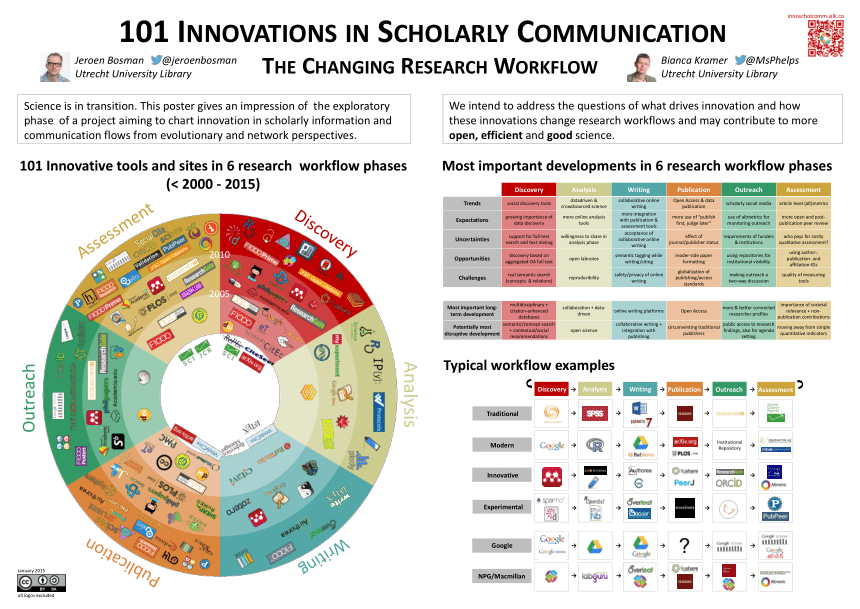
\includegraphics[width=0.75\linewidth]{101innovations} \\
\tiny{\href{https://s3-eu-west-1.amazonaws.com/pfigshare-u-previews/1863601/page_1_width_860.png}{Bosman, Kramer: 101 Innovations in Scholarly Communication}}

\end{frame}

%%%%%%%%%%%%%%%%%%%%%%%%%%%%%%%%%%%%%

\begin{frame}{Dann kann es los gehen.}

\begin{figure}
\begin{minipage}{0.59\linewidth}
\flushleft
Nun betrachten wir die Werkzeugkasten, die in der Informatik und in der Mathematik jeweils in den entsprechenden Phasen zur Verf\"ugung stehen.
\end{minipage}
\begin{minipage}{0.4\linewidth}
\centering
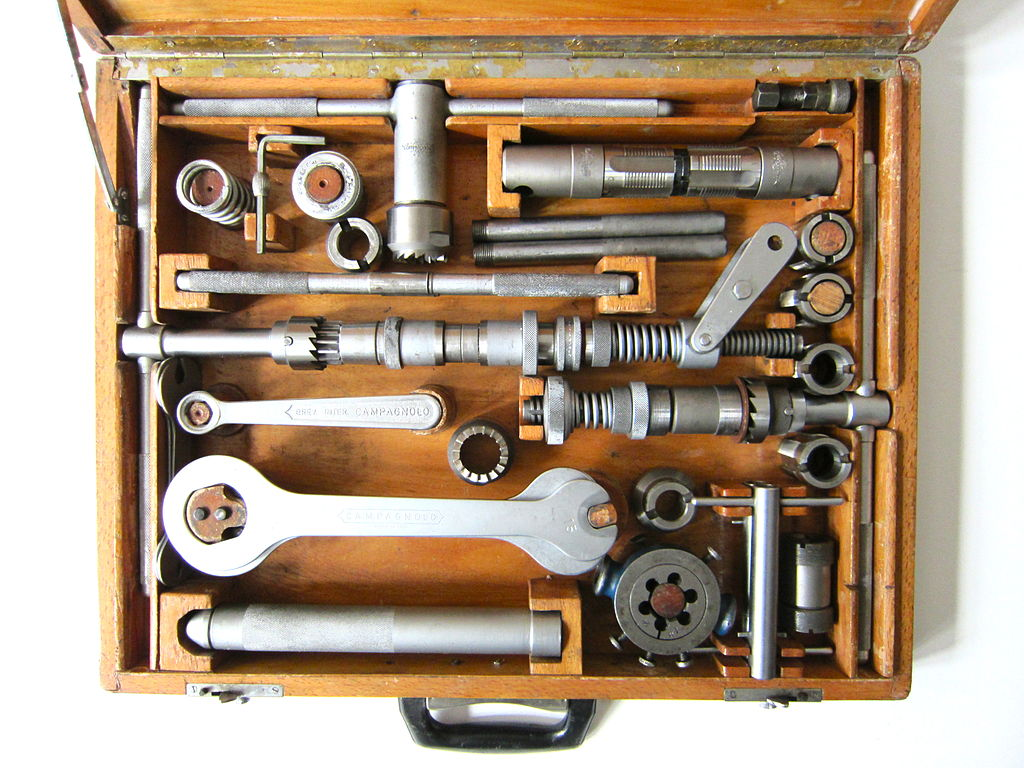
\includegraphics[width=0.8\linewidth]{toolbox} \\
\tiny{\href{https://upload.wikimedia.org/wikipedia/commons/thumb/3/3f/Campagnolo_1968_Tool_Kit_Wooden_Box.jpg/1024px-Campagnolo_1968_Tool_Kit_Wooden_Box.jpg}{Wikipedia}}
\end{minipage}
\end{figure}

\end{frame}

%%%%%%%%%%%%%%%%%%%%%%%%%%%%%%%%%%%%%

\section{Informatik}

%%%%%%%%%%%%%%%%%%%%%%%%%%%%%%%%%%%%%

\begin{frame}{1. Schritt: Entdecken (Discover) -- Werkzeuge}

\centering

\includegraphics[width=0.9\linewidth]{informatik_discover}

\end{frame}

%%%%%%%%%%%%%%%%%%%%%%%%%%%%%%%%%%%%%

\begin{frame}{1. Schritt: Entdecken (Discover) -- Google Scholar}

\begin{figure}
\begin{minipage}{0.7\linewidth}
\flushleft
\begin{itemize}[<+->]
\item Qualitativ und quantitativ beste akademische Suchmaschine.
\item Oft direkter Zugang zum Volltext (auch \"uber unser Angebot).
\item Datenschutz.
\item Urheberrecht.
\end{itemize}
\end{minipage}
\begin{minipage}{0.25\linewidth}
\centering

\includegraphics[width=0.9\linewidth]{GoogleScholarLogo}
\end{minipage}
\end{figure}

\end{frame}

%%%%%%%%%%%%%%%%%%%%%%%%%%%%%%%%%%%%%

\begin{frame}{1. Schritt: Entdecken (Discover) -- arXiv}

\begin{figure}
\begin{minipage}{0.7\linewidth}
\flushleft
\begin{itemize}[<+->]
\item Open Access Preprint-Server.
\item Nach Physik und Mathematik ist die Informatik das drittgr\"o\ss{}te Fach.
\item Sinnvoll, wenn man wei\ss{}, was man sucht (z. B. Autor, Titel).
\item Integriert in der Suche des TIB-Portals.
\end{itemize}
\end{minipage}
\begin{minipage}{0.25\linewidth}
\centering

\includegraphics[width=0.9\linewidth]{Arxiv}
\end{minipage}
\end{figure}

\end{frame}

%%%%%%%%%%%%%%%%%%%%%%%%%%%%%%%%%%%%%

\begin{frame}{1. Schritt: Entdecken (Discover) -- dblp}

\begin{figure}
\begin{minipage}{0.7\linewidth}
\flushleft
\begin{itemize}[<+->]
\item Gr\"o\ss{}te Bibliographie der Informatik.
\item Stand urspr\"unglich f\"ur \emph{Data Base and Logic Programming Bibliography}, nach ihrem Erfolg nun unter \emph{Digital Bibliography \& Library Project} bekannt.
\item Verzeichnet auch Konferenzbeitr\"age, die in der Informatik mindestens genauso wichtig wie Zeitschriftenbeitr\"age sind.
\item Freier Zugriff.
\item Open Source.
\end{itemize}
\end{minipage}
\begin{minipage}{0.25\linewidth}
\centering

\includegraphics[width=0.9\linewidth]{dblp}
\end{minipage}
\end{figure}

\end{frame}

%%%%%%%%%%%%%%%%%%%%%%%%%%%%%%%%%%%%%

\begin{frame}{1. Schritt: Entdecken (Discover) -- ACM Digital Library}

\begin{figure}
\begin{minipage}{0.7\linewidth}
\flushleft
\begin{itemize}[<+->]
\item \emph{Association for Computing Machinery (ACM)} erste und gr\"o\ss{}te Fachgesellschaft f\"ur die Informatik.
\item Die ACM ist Dachverband der wichtigsten Konferenzen und Zeitschriften in der Informatik.
\item \emph{ACM DL} stellt alle Ver\"offentlichungen seit Gr\"undung der ACM digital zur Verf\"ugung. 
\item Nur kostenpflichtiger Zugang.
\end{itemize}
\end{minipage}
\begin{minipage}{0.25\linewidth}
\centering

\includegraphics[width=0.9\linewidth]{acmdl}
\end{minipage}
\end{figure}

\end{frame}

%%%%%%%%%%%%%%%%%%%%%%%%%%%%%%%%%%%%%

\begin{frame}{1. Schritt: Entdecken (Discover) -- IEEE XPlore}

\begin{figure}
\begin{minipage}{0.7\linewidth}
\flushleft
\begin{itemize}[<+->]
\item Akademische Fachdatenbank zur Informatik, Elektrotechnik und Technik von der Fachgesellschaft f\"ur alle Technikbereiche, dem \emph{Institute of Electrical and Electronic Engineers}.
\item Nur kostenpflichtiger Zugang.
\item Obwohl INSPEC IEEE XPlore quasi enth\"alt, bei Umfrage und Nutzung abgeschlagen. 
\end{itemize}
\end{minipage}
\begin{minipage}{0.25\linewidth}
\centering

\includegraphics[width=0.9\linewidth]{IEEEXplore}
\end{minipage}
\end{figure}

\end{frame}

%%%%%%%%%%%%%%%%%%%%%%%%%%%%%%%%%%%%%

\begin{frame}{2. Schritt: Untersuchen (Analysis)}

\centering

\includegraphics[width=0.9\linewidth]{informatik_analysis}

\end{frame}

%%%%%%%%%%%%%%%%%%%%%%%%%%%%%%%%%%%%%

\begin{frame}{3. Schritt: Schreiben (Writing)}

\centering

\includegraphics[width=0.8\linewidth]{informatik_writing}

\end{frame}

%%%%%%%%%%%%%%%%%%%%%%%%%%%%%%%%%%%%%

\begin{frame}{4. Schritt: Ver\"offentlichen (Publication)}

\begin{figure}
\begin{minipage}{0.7\linewidth}
\flushleft
\begin{itemize}[<+->]
\item Sehr hohes Konkurrenzempfinden, daher gibt es ein gro\ss{}es Pflichtbewusstsein in renommierten Zeitschriften oder auf wichtigen Konferenzen zu ver\"offentlichen.
\item Monographien sind quasi ausgestorben.
\item Zum Teil sehr industrienah.
\item Open Access gew\"unscht, aber schwierig umzusetzen.
\end{itemize}
\end{minipage}
\begin{minipage}{0.25\linewidth}
\centering

\includegraphics[width=0.9\linewidth]{OA}
\end{minipage}
\end{figure}

\end{frame}

%%%%%%%%%%%%%%%%%%%%%%%%%%%%%%%%%%%%%

\begin{frame}{5. Schritt: Verbreiten (Outreach)}

\begin{figure}
\begin{minipage}{0.6\linewidth}
\flushleft
\begin{itemize}[<+->]
\item Hochrangige Konferenzen (ACM).
\item arXiv.
\item Homepage.
\item Social Media.
\end{itemize}
\end{minipage}
\begin{minipage}{0.39\linewidth}
\centering
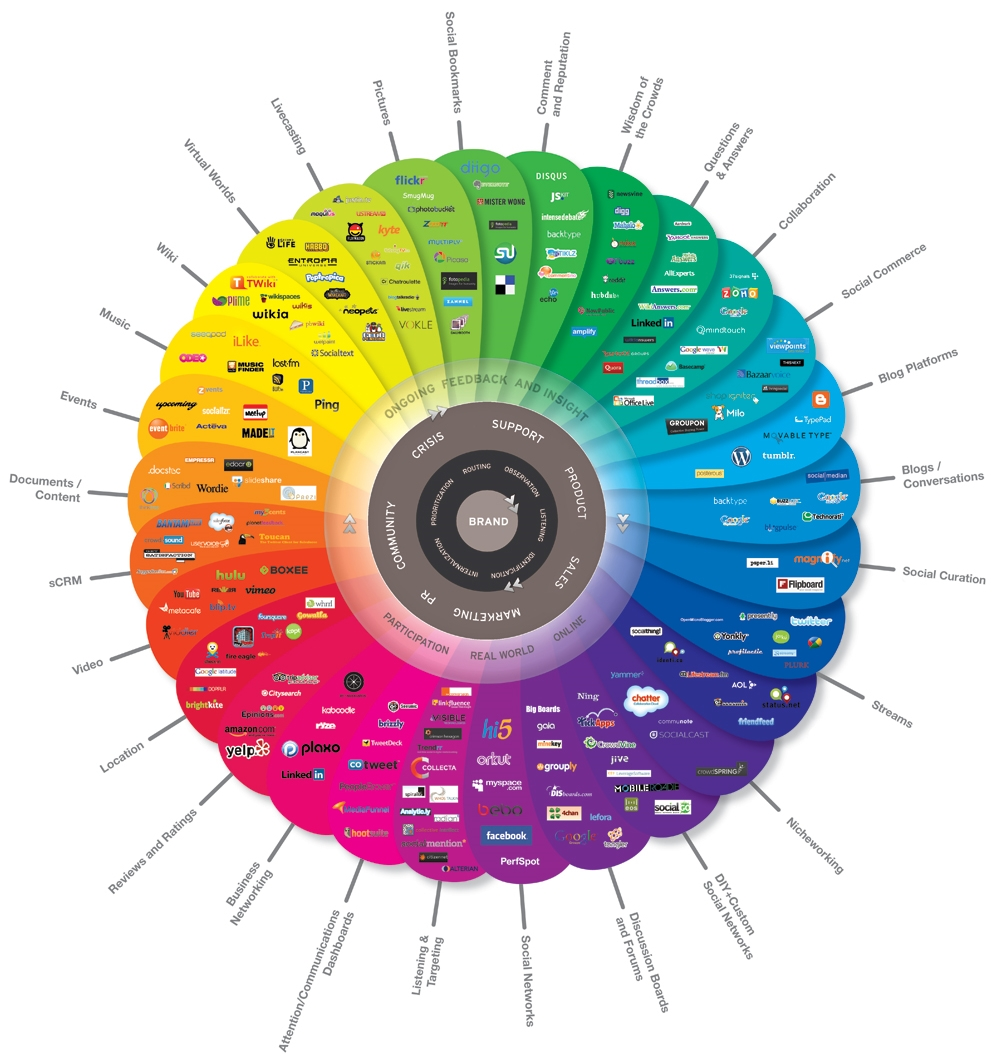
\includegraphics[width=0.9\linewidth]{SocialMedia} \\
\tiny{\href{https://upload.wikimedia.org/wikipedia/commons/7/7c/Conversationprism.jpeg}{Wikipedia}}
\end{minipage}
\end{figure}

\end{frame}

%%%%%%%%%%%%%%%%%%%%%%%%%%%%%%%%%%%%%

\begin{frame}{6. Schritt: Bewerten (Assessment)}

\begin{figure}
\begin{minipage}{0.6\linewidth}
\flushleft
\begin{itemize}[<+->]
\item Impact Factor.
\item Hirsch-Index.
\item Nachweis in den gro\ss{}en Datenbanken (ACM, IEEE).
\item F\"orderquellen.
\item Nachnutzung in Software-Firmen.
\end{itemize}
\end{minipage}
\begin{minipage}{0.39\linewidth}
\centering
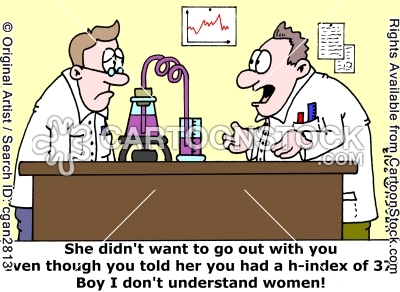
\includegraphics[width=0.9\linewidth]{hindex} \\
\tiny{\href{https://scepticemia.files.wordpress.com/2014/07/dating-scientist-date-girlfriend-boyfriend-experiment-cgan2813l-jpg.png}{Quelle}}
\end{minipage}
\end{figure}

\end{frame}

%%%%%%%%%%%%%%%%%%%%%%%%%%%%%%%%%%%%%

\section{Mathematik}

%%%%%%%%%%%%%%%%%%%%%%%%%%%%%%%%%%%%%

\begin{frame}{1. Schritt: Entdecken (Discover) -- Werkzeuge}

\centering

\includegraphics[width=0.9\linewidth]{mathematik_discover}

\end{frame}

%%%%%%%%%%%%%%%%%%%%%%%%%%%%%%%%%%%%%

\begin{frame}{1. Schritt: Entdecken (Discover) -- Google Scholar}

\begin{figure}
\begin{minipage}{0.7\linewidth}
\flushleft
\begin{itemize}[<+->]
\item Qualitativ und quantitativ beste akademische Suchmaschine.
\item Oft direkter Zugang zum Volltext (auch \"uber unser Angebot).
\item Datenschutz.
\item Urheberrecht.
\end{itemize}
\end{minipage}
\begin{minipage}{0.25\linewidth}
\centering

\includegraphics[width=0.9\linewidth]{GoogleScholarLogo}
\end{minipage}
\end{figure}

\end{frame}

%%%%%%%%%%%%%%%%%%%%%%%%%%%%%%%%%%%%%

\begin{frame}{1. Schritt: Entdecken (Discover) -- arXiv}

\begin{figure}
\begin{minipage}{0.7\linewidth}
\flushleft
\begin{itemize}[<+->]
\item Open Access Preprint-Server.
\item Nach Physik ist die Mathematik das zweitgr\"o\ss{}te Fach.
\item Sinnvoll, wenn man wei\ss{}, was man sucht (z. B. Autor, Titel).
\item Integriert in der Suche des TIB-Portals.
\end{itemize}
\end{minipage}
\begin{minipage}{0.25\linewidth}
\centering

\includegraphics[width=0.9\linewidth]{Arxiv}
\end{minipage}
\end{figure}

\end{frame}

%%%%%%%%%%%%%%%%%%%%%%%%%%%%%%%%%%%%%

\begin{frame}{1. Schritt: Entdecken (Discover) -- zbMATH}

\begin{figure}
\begin{minipage}{0.7\linewidth}
\flushleft
\begin{itemize}[<+->]
\item Nachweise und zum Teil Direktzugang zu (fast) allen Ver\"offentlichungen in der Mathematik seit dem 19. Jahrhundert.
\item Mitherausgeber der Fachklassifizierung \emph{Mathematics Subject Classification}.
\item Kostenfreier Webdienst mit eingeschr�nkten Funktionalit\"aten.
\item Gr\"o\ss{}te Autorendatenbank in der Mathematik.
\item Formelsuche und Software-Nachweissystem.
\end{itemize}
\end{minipage}
\begin{minipage}{0.25\linewidth}
\centering

\includegraphics[width=0.9\linewidth]{zbmath_logo}
\end{minipage}
\end{figure}

\end{frame}

%%%%%%%%%%%%%%%%%%%%%%%%%%%%%%%%%%%%%

\begin{frame}{1. Schritt: Entdecken (Discover) -- MathSciNet}

\begin{figure}
\begin{minipage}{0.7\linewidth}
\flushleft
\begin{itemize}[<+->]
\item U.S.-amerikanisches Pendant des zbMATH (derselbe Gr\"undungsvater).
\item Mitherausgeber der Fachklassifizierung \emph{Mathematics Subject Classification}.
\item \emph{Mathematical citation quotient} als Alternative zum Impact Factor.
\item Nur kostenpflichtiger Zugang.
\end{itemize}
\end{minipage}
\begin{minipage}{0.25\linewidth}
\centering

\includegraphics[width=0.9\linewidth]{mathscinet-logo}
\end{minipage}
\end{figure}

\end{frame}

%%%%%%%%%%%%%%%%%%%%%%%%%%%%%%%%%%%%%

\begin{frame}{1. Schritt: Entdecken (Discover) -- Wolfram Alpha}

\begin{figure}
\begin{minipage}{0.7\linewidth}
\flushleft
\begin{itemize}[<+->]
\item Semantische Suchmaschine f\"ur Mathematik (gilt als bislang beste semantische Suchmaschine der Welt).
\item Basiert auf Mathematica.
\item Nicht auf Literaturrecherche, sondern auf (mathematik-)wissenschaftliche Fragestellungen spezialisiert.
\item Kostenfreier Webdienst mit eingeschr�nkten Funktionalit\"aten.
\item \href{https://www.wolframalpha.com/}{Wolfram Alpha zum Ausprobieren.}
\end{itemize}
\end{minipage}
\begin{minipage}{0.25\linewidth}
\centering

\includegraphics[width=0.9\linewidth]{wolframalpha-logo}
\end{minipage}
\end{figure}

\end{frame}

%%%%%%%%%%%%%%%%%%%%%%%%%%%%%%%%%%%%%

\begin{frame}{2. Schritt: Untersuchen (Analysis)}

\centering
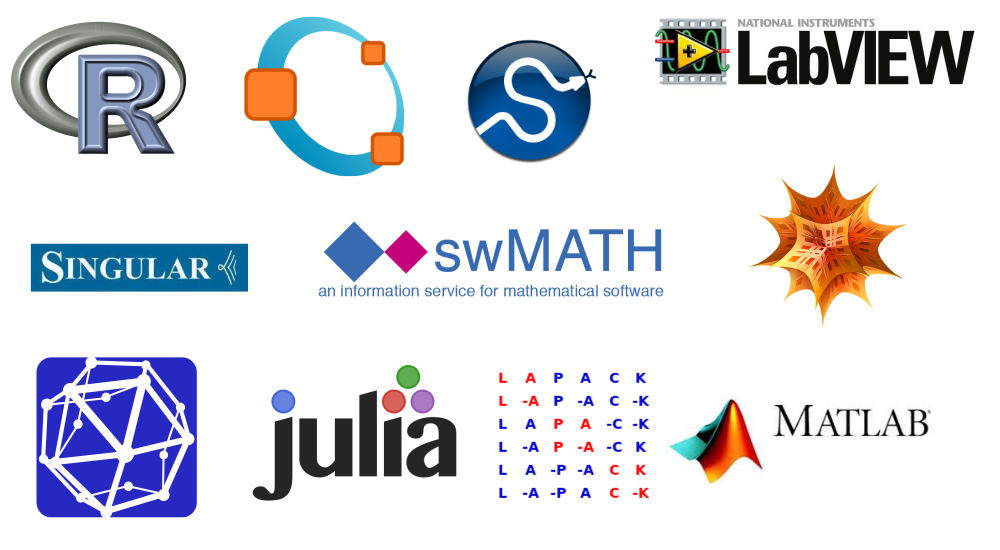
\includegraphics[width=0.9\linewidth]{mathematik_analysis}

\end{frame}

%%%%%%%%%%%%%%%%%%%%%%%%%%%%%%%%%%%%%

\begin{frame}{3. Schritt: Schreiben (Writing)}

\centering

\includegraphics[width=0.8\linewidth]{mathematik_writing}

\end{frame}

%%%%%%%%%%%%%%%%%%%%%%%%%%%%%%%%%%%%%

\begin{frame}{4. Schritt: Ver\"offentlichen (Publication)}

\begin{figure}
\begin{minipage}{0.7\linewidth}
\flushleft
\begin{itemize}[<+->]
\item Open Access weit verbreitet.
\item 80\% aller Publikationen in der Mathematik werden auf arXiv (zus\"atzlich) ver\"offentlicht.
\item Offen f\"ur alternative Publikationsformen.
\end{itemize}
\end{minipage}
\begin{minipage}{0.25\linewidth}
\centering

\includegraphics[width=0.9\linewidth]{OA}
\end{minipage}
\end{figure}

\end{frame}

%%%%%%%%%%%%%%%%%%%%%%%%%%%%%%%%%%%%%

\begin{frame}{5. Schritt: Verbreiten (Outreach)}

\begin{figure}
\begin{minipage}{0.6\linewidth}
\flushleft
\begin{itemize}[<+->]
\item arXiv.
\item Homepage.
\item Social Media.
\end{itemize}
\end{minipage}
\begin{minipage}{0.39\linewidth}
\centering
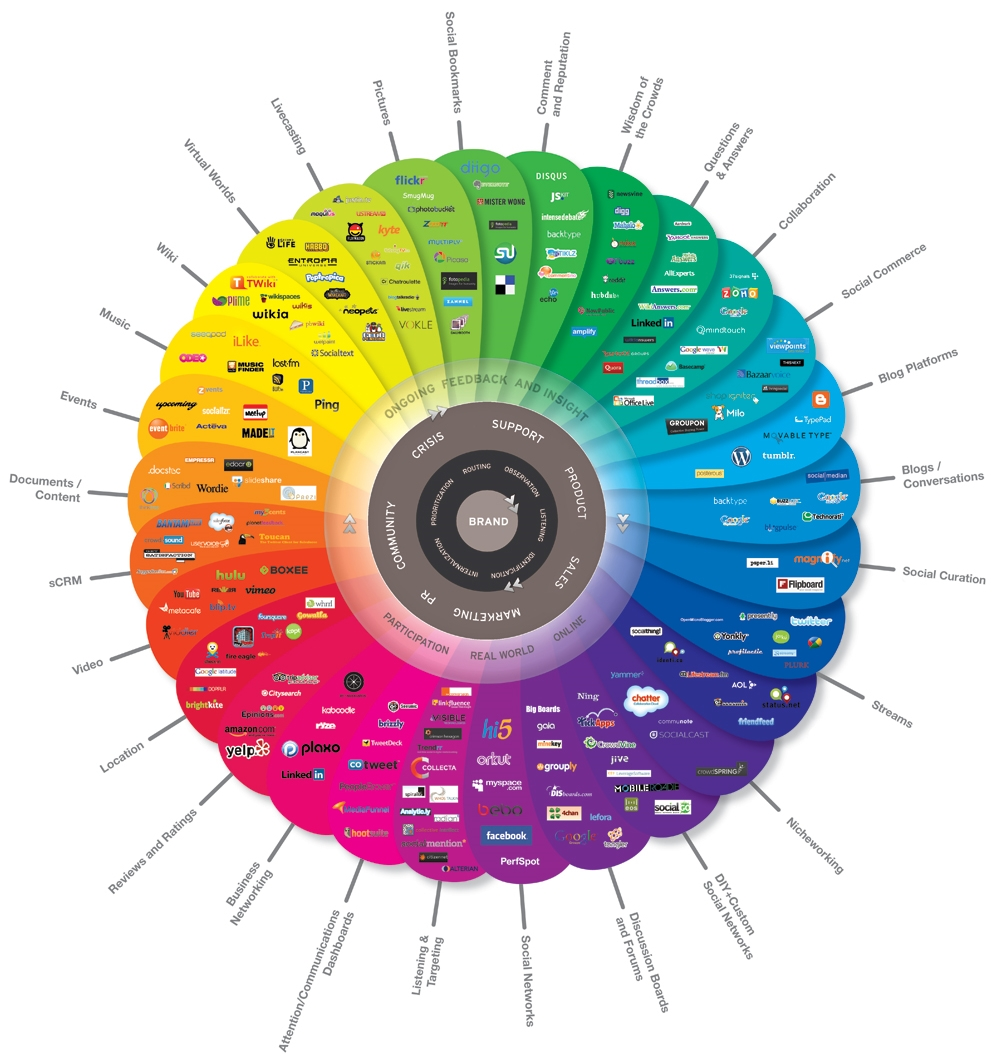
\includegraphics[width=0.9\linewidth]{SocialMedia} \\
\tiny{\href{https://upload.wikimedia.org/wikipedia/commons/7/7c/Conversationprism.jpeg}{Wikipedia}}
\end{minipage}
\end{figure}

\end{frame}

%%%%%%%%%%%%%%%%%%%%%%%%%%%%%%%%%%%%%

\begin{frame}{6. Schritt: Bewerten (Assessment)}

\begin{figure}
\begin{minipage}{0.7\linewidth}
\flushleft
\begin{itemize}[<+->]
\item \glqq{}Die Halbwertszeit mathematischen Wissens wird durch den Impact Factor nicht korrekt wiedergegeben.\grqq{} (Fields-Medaillisten David Mumford und Timothy Gowers)
\item \href{https://en.wikipedia.org/wiki/Mathematical_Reviews\#Mathematical_citation_quotient}{Mathematical citation quotient}.
\item Personenkult.
\end{itemize}
\end{minipage}
\begin{minipage}{0.29\linewidth}
\centering

\includegraphics[width=0.9\linewidth]{2014_impact_factor} \\
\tiny{\href{http://www.enago.de/blog/wp-content/uploads/2014/06/2014_impact_factor.png}{Quelle}}
\end{minipage}
\end{figure}

\end{frame}

%%%%%%%%%%%%%%%%%%%%%%%%%%%%%%%%%%%%%

\begin{frame}{Bei Risiken und Nebenwirkungen fragen Sie \ldots}

\begin{figure}
\begin{minipage}{0.7\linewidth}
\flushleft
\begin{itemize}[<+->]
\item Kommilitonen.
\item Fachschaft.
\item Dozent.
\item Google.
\item \alert{Bibliothek.}
\end{itemize}
\end{minipage}
\begin{minipage}{0.29\linewidth}
\centering

\includegraphics[width=0.9\linewidth]{dreifragezeichen} \\
\tiny{\href{https://i.ytimg.com/vi/AjXOdZKjQXk/maxresdefault.jpg}{Quelle}}
\end{minipage}
\end{figure}

\end{frame}

%%%%%%%%%%%%%%%%%%%%%%%%%%%%%%%%%%%%%

\section{Fachinformationsdienst Mathematik}

%%%%%%%%%%%%%%%%%%%%%%%%%%%%%%%%%%%%%

\begin{frame}{Fachinformationsdienst Mathematik -- Ziel (1/2)}

Ziel der DFG-gef\"orderten \glqq{}Fachinformationsdienste (FID) f\"ur die Wissenschaft\grqq{} ist es,

\vspace{\baselineskip}

\begin{bfseries}
\glqq{}Wissenschaftlerinnen und Wissenschaftlern aller Fachrichtungen in Deutschland unabh\"angig vom Standort ihrer T\"atigkeit einen m\"oglichst schnellen und direkten Zugriff auf Spezialliteratur und forschungsrelevante Informationen zu erm\"oglichen\grqq{}
\end{bfseries}

\vspace{\baselineskip}

Quelle: \href{http://www.dfg.de/foerderung/programme/infrastruktur/lis/lis_foerderangebote/fachinformationsdienste_wissenschaft/}{Informationen zum F\"orderprogramm FID}

\end{frame}

%%%%%%%%%%%%%%%%%%%%%%%%%%%%%%%%%%%%%

\begin{frame}{Fachinformationsdienst Mathematik -- Ziel (2/2)}

Grunds\"atze der DFG-gef\"orderten \glqq{}Fachinformationsdienste f\"ur die Wissenschaft\grqq{}:

\begin{bfseries}
\begin{enumerate}
\item \glqq{}Bei der Ausgestaltung der Fachinformationsdienste stehen die Forschungsinteressen der F\"acher im Mittelpunkt.\grqq{}
\item \glqq{}Die Leistungen der Fachinformationsdienste grenzen sich von den Grundaufgaben wissenschaftlicher Bibliotheken ab und stellen einen Mehrwert gegen\"uber bestehenden Angeboten dar.\grqq{}
\end{enumerate}
\end{bfseries}

Quelle: \href{http://www.dfg.de/formulare/12_102/12_102_de.pdf}{Richtlinien FID}

\end{frame}

%%%%%%%%%%%%%%%%%%%%%%%%%%%%%%%%%%%%%

\begin{frame}{Fachinformationsdienst Mathematik -- Projektpartner}

\centering

\includegraphics[width=0.9\linewidth]{fid}

\end{frame}

%%%%%%%%%%%%%%%%%%%%%%%%%%%%%%%%%%%%%

\begin{frame}{Fachinformationsdienst Mathematik -- Projektplan}

\begin{enumerate}
\item Konzeption
\item \textbf{Kooperation mit der Fachcommunity (TIB f\"ur Angewandte Mathematik)}
\item Erwerbung und Lizenzierung
\item Aufbau eines digitalen Mathematiker-Archivs
\item \textbf{Neue Dienstleistungen f\"ur die Mathematik: \textit{Maths Beyond Text} (TIB)}
\item Digitalisierung
\item FID-Web-Portal
\item \textbf{Workshops (TIB f\"ur Angewandte Mathematik)}
\item Projektmanagement \& \"Offentlichkeitsarbeit
\end{enumerate}

\end{frame}

%%%%%%%%%%%%%%%%%%%%%%%%%%%%%%%%%%%%%

\begin{frame}{Fachinformationsdienst Mathematik -- \textit{Maths Beyond Text}}

Forschungsdaten hatten schon immer eine gro\ss{}e Bedeutung in der Mathematik. Dass sie nicht ver\"offentlicht wurden, war eine Frage der Logistik. Mit der Digitalisierung m\"ussen alle Forschungsdaten publiziert werden, um der guten wissenschaftlichen Praxis zu entsprechen:

\begin{itemize}
\item Verf\"ugbarkeit.
\item Nachnutzbarkeit.
\item Reproduzierbarkeit.
\end{itemize}

Nach einer Umfrage sollten wir mit Software als h\"aufigstem Forschungsdatum beginnen.

\end{frame}

%%%%%%%%%%%%%%%%%%%%%%%%%%%%%%%%%%%%%

\begin{frame}{Fachinformationsdienst Mathematik -- Mehr Informationen}

\begin{figure}
\begin{minipage}{0.7\linewidth}
\flushleft
\begin{itemize}
\item \href{http://fidmath.de/}{Portal des FID Mathematik.}
\item \href{https://github.com/runnwerth/}{Vortr\"age zu unserer Arbeit im FID und mehr.}
\item \href{http://mathematik.fid-lizenzen.de/}{Lizenzen des FID Mathematik.}
\item \href{https://twitter.com/FIDMathematik}{FID Mathematik auf Twitter.}
\end{itemize}
\end{minipage}
\begin{minipage}{0.29\linewidth}
\centering

\includegraphics[width=0.9\linewidth]{fidlogo}
\end{minipage}
\end{figure}

\end{frame}

%%%%%%%%%%%%%%%%%%%%%%%%%%%%%%%%%%%%%

\section{Anregungen \& Fragen}

%%%%%%%%%%%%%%%%%%%%%%%%%%%%%%%%%%%%%

\begin{frame}{Anregungen \& Fragen}

\begin{figure}
\begin{minipage}{0.4\linewidth}
Mila Runnwerth \\
Tel.: +49 511 762 3979 \\
\href{mailto:mila.runnwerth@tib.eu}{mila.runnwerth@tib.eu} \\

\href{https://github.com/runnwerth/2016_FoBi_Fachrecherche}{Hier sind die Folien.}
\end{minipage}
\begin{minipage}{0.5\linewidth}
\centering
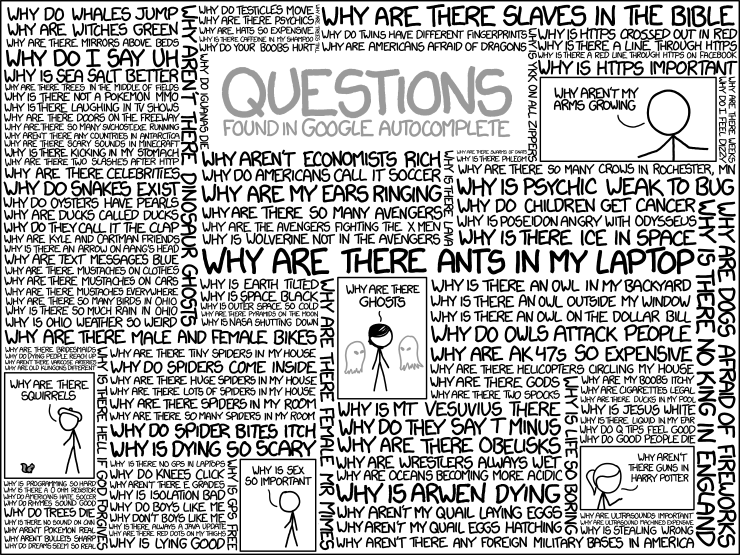
\includegraphics[width=0.9\linewidth]{questions} \\
\tiny{\href{https://xkcd.com/1256/}{Quelle}}
\end{minipage}
\end{figure}


\end{frame}

%%%%%%%%%%%%%%%%%%%%%%%%%%%%%%%%%%%%%

\end{document}
